\documentclass[hyperref={pdfpagemode=FullScreen,colorlinks=true}]{beamer}
\usepackage{concrete} % une police qui va bien pour l'écran

\usepackage[utf8]{inputenc}
\usepackage[T1]{fontenc}
\usepackage[french]{babel}
\usetheme{default}
\title{Le titre de la présentation}
\author{G. \textsc{Faccanoni}}
\institute{IMATH-UTLN}
\setbeamertemplate{navigation symbols}{}
\begin{document}
\begin{frame}[plain]
\maketitle
\end{frame}
\begin{frame}
Le texte de ma diapo.
\end{frame}

\begin{frame}
\frametitle{Titre à la diapo}
Bla bla bla \structure{bla bla bla bla} bla bla
Bla bla \alert{bla bla} bla bla bla bla bla

\end{frame}

\begin{frame}
\frametitle{Titre à la diapo}
\begin{columns}
\begin{column}{0.7\textwidth}
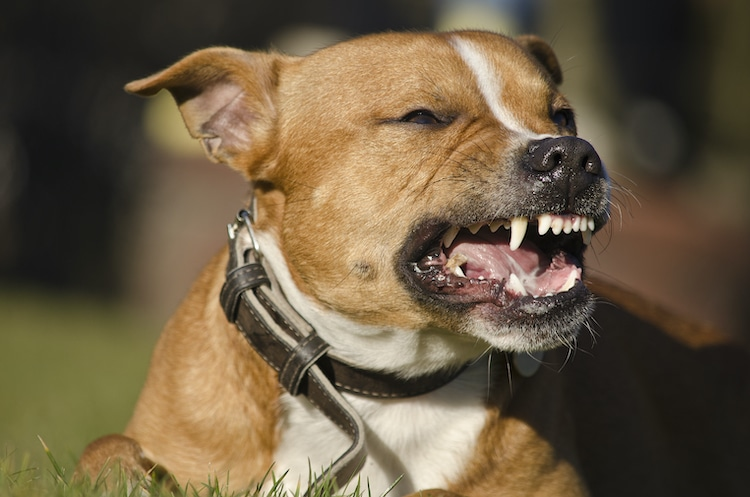
\includegraphics[width=\textwidth]{dog}
\end{column}
\begin{column}{0.4\textwidth}
\begin{itemize}
\item wouf
\item wouf
\end{itemize}
\end{column}
\end{columns}
\end{frame}
\begin{frame}
\textbf<1>{Blah!} 
\textbf<2>{bleh!} 
\textbf<3>{blih!}
\begin{itemize}
\item<3-> Liberte
\item<2-> Egalite
\item<1-> Fraternite
\end{itemize}
\end{frame}
\begin{frame}
\begin{itemize}
\item avec espace reserve:
	{\ttfamily
		\uncover<2>{blabla} \uncover<3>{bleble} \uncover<4>{blibli}
	}
\item Sans espece reserver:
	{\ttfamily
	  \only<2>{blabla} \only<3>{bleble} \only<4>{blibli}
	  }	
\end{itemize}
\end{frame}
\end{document}